\section{Affichage et visualisation des cours}
%http://www.simpleentrepreneur.com/2007/06/07/16-librairies-et-scripts-pour-generer-des-graphiques-sur-internet/
%http://www.fusioncharts.com/goodies/fusioncharts-free/
%http://docs.fusioncharts.com/free/#_ga=1.124638285.613042136.1459322699
%https://fr.wikipedia.org/wiki/Adobe_Flash

L'un des objectifs de notre projet étant de fournir à l'utilisateur une IHM pour visualiser les cours ainsi que des indicateurs financiers via l'analyse technique que nous verrons dans le chapitre suivant, nous avons besoin d'afficher des graphes et autres diagrammes.
Par exemple, nous pourrions vouloir afficher l'historique d'un cours sur une période ou encore visualiser la répartition des actifs d'un portefeuille sous forme diagramme en camembert. Le graphique doit donc être afficher sur une page web sachant que nous utilisons une plateforme Java EE.\\

Pour cela, plusieurs possibilités s'offraient à nous :
\begin{itemize}
 \item Publier les graphiques en 'Flash',
 \item Générer des graphes sous forme d'image puis les afficher,
 \item Utiliser une générateur Javascript permettant l'affichage de graphiques.
\end{itemize}

Nous allons présenter un exemple de chacune de ces possibilités que nous aurions pu utiliser puis nous expliquerons notre choix.

%-------------------------------------------------------------------%
%------------------------FusionCharts-------------------------------%
%-------------------------------------------------------------------%
\subsection{Graphiques en Flash : FusionCharts Free}

\subsubsection{Présentation de Flash}
Flash est une technologie qui permet de manipuler des graphiques vectoriels, des bitmaps et certains scripts utilisés dans les applications web, les jeux et les vidéos. L'avantage de Flash est qu'il est répandu sur de nomreux logiciels et nombreux systèmes d'exploitation.\\

Les fichiers Flash ont pour extension '.swf' et peuvent être inclus dans une page web puis lus par le plugin Flash du navigateur. Sinon, ils peuvent être interprétés de manière indépendante dans le lecteur Flash Player.\\
Aujourd'hui, le plugin Flash est la technologie la plus utilisée dans les navigateurs web pour afficher du contenu multimédia. On se pose néanmoins la question de son remplacement par HTML5 dans un futur proche.\\
Le lecteur Flash permettant la lecture des fichiers multimédias a été développé par Adobe Systems et est compatible avec la plupart des systèmes d'exploitation et navigateurs.
\begin{figure}[H]
  \center
  
\includegraphics[scale=0.4]{../graph/flashAdobe.jpg}
  \caption{Adobe Flash Player - \url{http://www.adobe.com/fr/products/flashplayer.html}}
\end{figure}
D'autres projets de lecteurs Flash existent mais ne sont pas aboutis.

\subsubsection{FusionCharts Free}
FusionCharts Free est un composant open-source permettant d'intégrer des graphes intéractifs et animés dans une application web. Il utilise la technologie Flash décrite précédemment. Il existe une version gratuite 'FusionCharts Free', c'est un logiciel multiplate-forme qui peut être implémenté avec toute sorte de technologies comme PHP, .NET, Python, JSP ou même un simple HTML.\\

On s'intéresse à la version qui utilise les JSP car c'est celle que l'on pourrait utiliser dans notre projet.
On peut trouver les guides et téléchargements nécessaires sur le site Internet :
\begin{figure}[H]
  \center
  
\includegraphics[scale=0.7]{../graph/fusionCharts.png}
  \caption{FusionCharts Free - \url{http://www.fusioncharts.com/goodies/fusioncharts-free/}}
\end{figure}

Les étapes pour la mise en place d'un graphe sur une page web sont les suivantes :
\begin{enumerate}
 \item \textbf{Mettre en place les données :} possibilité de fournir les données sous forme JSON ou XML. Cela peut être une chaîne de caractères ou un fichier. Voici un exemple en XML que nous pourrions utiliser et qui serait placé dans un fichier Donnees.xml :
\begin{lstlisting}[language=XML]
<graph caption="Revenus trimestriels 2015" xaxisname="Trimestres" yaxisname="Revenus (euros)">
    <set label="T1" value="420000" />
    <set label="T2" value="810000" />
    <set label="T3" value="720000" />
</graph>
\end{lstlisting}
 \item \textbf{Inclure le code HTML pour intégrer l'objet Flash et fournir les paramètres nécessaires :} cette étape est fourni par le développeur dans un fichier JSP téléchargeable sur le site (FusionChartsHTMLRenderer.jsp). Il suffira alors d'inclure le fichier dans la page web où l'on souhaite afficher un graphe. Il ne reste plus donc qu'à intégrer le code suivant dans les balises HTML de notre JSP.\\
 Le paramètre chartSWF précise la forme de graphe utilisée (ici un colonne en 3D), on place nos données dans strURL ou strXML suivant si on utilise l'URL d'un fichier ou si on défini dans une variable locale les données.
 Chaque graphe d'une page doit avoir un ID unique, que l'on choisit dans le paramètre chartId. On peut également choisir la hauteur et la largeur du graphe qui s'affichera.
\begin{lstlisting}[language=HTML]
<jsp:include page="../Includes/FusionChartsHTMLRenderer.jsp" flush="true">
    <jsp:param name="chartSWF" value="../../FusionCharts/FCF_Column3D.swf" />
    <jsp:param name="strURL" value="Data/Donnes.xml" />
    <jsp:param name="strXML" value="" />
    <jsp:param name="chartId" value="graphe1" />
    <jsp:param name="chartWidth" value="600" />
    <jsp:param name="chartHeight" value="300" />
</jsp:include>
\end{lstlisting} 
 \item \textbf{Visualiser le graphe sur la page web :} avec les exemples précédents et des données un peu plus détaillées, on obtiendrait un graphe comme le suivant.
\begin{figure}[H]
  \center
  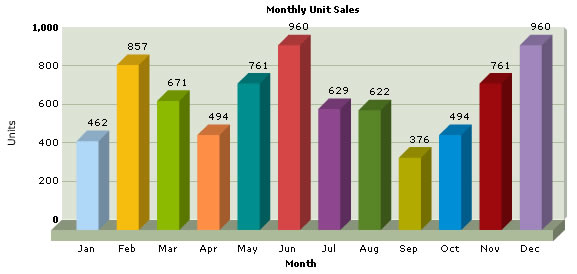
\includegraphics[scale=0.7]{../graph/fusionChartsExemple.jpg}
  \caption{Exemple de graphe en colonne 3D avec FusionCharts Free - \url{http://docs.fusioncharts.com/free/}}
\end{figure}
\end{enumerate}




%-------------------------------------------------------------------%
%------------------------JFreeChart---------------------------------%
%-------------------------------------------------------------------%
\subsection{Images de graphes : JFreeChart}

%-------------------------------------------------------------------%
%------------------------GoogleChart--------------------------------%
%-------------------------------------------------------------------%
\subsection{Javascript : API Google Chart}

%-------------------------------------------------------------------%
%------------------------notrechoix---------------------------------%
%-------------------------------------------------------------------%
\subsection{Notre choix}